\documentclass[11pt,a4paper]{article}

\usepackage[T1]{fontenc}
\usepackage[utf8]{inputenc}
\usepackage[ngerman]{babel}
\usepackage{lmodern}
\usepackage{microtype}
\usepackage[a4paper,landscape,margin=2.5cm]{geometry}
\usepackage{graphicx}
\usepackage{xcolor}
\usepackage{hyperref}
\usepackage{multicol}
\usepackage{float}
\usepackage{fancyhdr}
\usepackage{csquotes}
\usepackage{adjustbox}
\usepackage{pdflscape}
\usepackage[acronym]{glossaries}
\usepackage[backend=biber,style=authoryear,sorting=nyt]{biblatex}
\addbibresource{references.bib}
% Acronyms
\newacronym{zvv}{ZVV}{Zürcher Verkehrsverbund}
\newacronym{nvz}{NVZ}{Nebenverkehrszeit}
\newacronym{oev}{öV}{öffentlicher Verkehr}
\newacronym{miv}{MIV}{motorisierter Individualverkehr}
\newacronym{bfs}{BFS}{Bundesamt für Statistik}
\newacronym{are}{ARE}{Bundesamt für Raumentwicklung}
\newacronym{sbb}{SBB}{Schweizerische Bundesbahnen}
\newacronym{zsg}{ZSG}{Zürichsee-Schifffahrtsgesellschaft}
\newacronym{roi}{ROI}{Return on Investment}
\newacronym{ga}{GA}{Generalabonnement}

% Glossarbegriffe
\newglossaryentry{doublediam}{
  name={Double Diamond},
  description={Vom British Design Council (2005) entwickeltes Modell des Design-Thinking-Prozesses, das vier Phasen (Discover, Define, Develop, Deliver) in zwei aufeinanderfolgenden Rauten visualisiert}
}

\newglossaryentry{designthinking}{
  name={Design Thinking},
  description={Nutzerzentrierter Innovations- und Probleml\"osungsansatz, der iteratives Vorgehen, Empathie f\"ur die Zielgruppe und experimentelles Prototyping verbindet}
}

\newglossaryentry{pov}{
  name={Point of View},
  description={Pr\"azise Problemformulierung im Design Thinking, die das noch unerf\"ullte Bed\"urfnis einer bestimmten Nutzergruppe beschreibt}
}

\makeglossaries

% Leichte Pastellfarben pro Double-Diamond-Phase
\definecolor{identifyPastel}{HTML}{FFF4CC}
\definecolor{discoverPastel}{HTML}{DCEEFF}
\definecolor{definePastel}{HTML}{E5F4E3}
\definecolor{developPastel}{HTML}{FFE8D6}
\definecolor{deliverPastel}{HTML}{EAF0F7}
\definecolor{defaultPastel}{HTML}{F1E7FF}

% Reusable style for all mindmap-like graphics in this report.
\usepackage{tikz}
\usetikzlibrary{arrows.meta,positioning,calc}

\definecolor{mmInk}{HTML}{000000}

\tikzset{
  mm canvas/.style={draw=none, fill=none},
  mm node outline/.style={
    draw=mmInk,
    line cap=round,
    line join=round,
    line width=0.55pt
  },
  mm curve/.style={
    draw=mmInk,
    line cap=round,
    line join=round,
    line width=0.45pt
  },
  mm central/.style={
    mm node outline,
    circle,
    minimum size=38mm,
    align=center,
    fill=identifyPastel,
    text=mmInk,
    font=\normalsize\itshape
  },
  mm topic/.style={
    mm node outline,
    rounded corners=2pt,
    minimum width=30mm,
    minimum height=8.5mm,
    align=center,
    fill=identifyPastel,
    text=mmInk,
    font=\normalsize\itshape,
    inner xsep=2.5mm
  },
  mm sub/.style={
    mm node outline,
    rounded corners=2pt,
    minimum width=26mm,
    minimum height=8mm,
    align=center,
    fill=identifyPastel,
    text=mmInk,
    font=\normalsize\itshape,
    inner xsep=2mm
  },
  mm topic red/.style={mm topic},
  mm topic orange/.style={mm topic},
  mm topic greyblue/.style={mm topic},
  mm topic purple/.style={mm topic},
  mm topic magenta/.style={mm topic},
  mm topic brown/.style={mm topic},
  mm topic dark/.style={mm topic},
  mm sub red/.style={mm sub},
  mm sub orange/.style={mm sub},
  mm sub greyblue/.style={mm sub},
  mm sub purple/.style={mm sub},
  mm sub magenta/.style={mm sub},
  mm sub brown/.style={mm sub},
  mm sub dark/.style={mm sub},
  mm link red/.style={mm curve},
  mm link orange/.style={mm curve},
  mm link greyblue/.style={mm curve},
  mm link purple/.style={mm curve},
  mm link magenta/.style={mm curve},
  mm link brown/.style={mm curve},
  mm link dark/.style={mm curve},
  mm sublink/.style={mm curve}
}


% Spaltenabstand vergrößern
\setlength{\columnsep}{1.5cm}
\setlength{\headheight}{14pt}

\hypersetup{
  colorlinks=true,
  linkcolor=blue!50!black,
  urlcolor=blue!50!black,
  pdftitle={Kurt Kreuz und Quer},
  pdfauthor={Martina Fasano, Simona Venzin, Dominic Hüppi}
}

\title{Kurt Kreuz und Quer}
\author{Martina Fasano, Simona Venzin, Dominic Hüppi}
\date{\today}

\newcommand{\worktitle}{Kurt Kreuz und Quer}

% Inhaltsverzeichnis nur bis Ebene X.Y
\setcounter{tocdepth}{2}

\makeatletter
\newcommand{\printtwocolumntoc}{%
  \markboth{\contentsname}{\contentsname}
  \section*{\contentsname}
  \begin{multicols}{2}
    \@starttoc{toc}
  \end{multicols}
}
\makeatother

\pagestyle{fancy}
\fancyhf{}
\fancyhead[L]{\worktitle}
\fancyhead[R]{\nouppercase{\leftmark}}
\fancyfoot[C]{\thepage}
\renewcommand{\headrulewidth}{0.4pt}
\renewcommand{\footrulewidth}{0pt}

\begin{document}

\pagecolor{defaultPastel}

\maketitle
\begin{center}
  \vspace{0.8cm}
  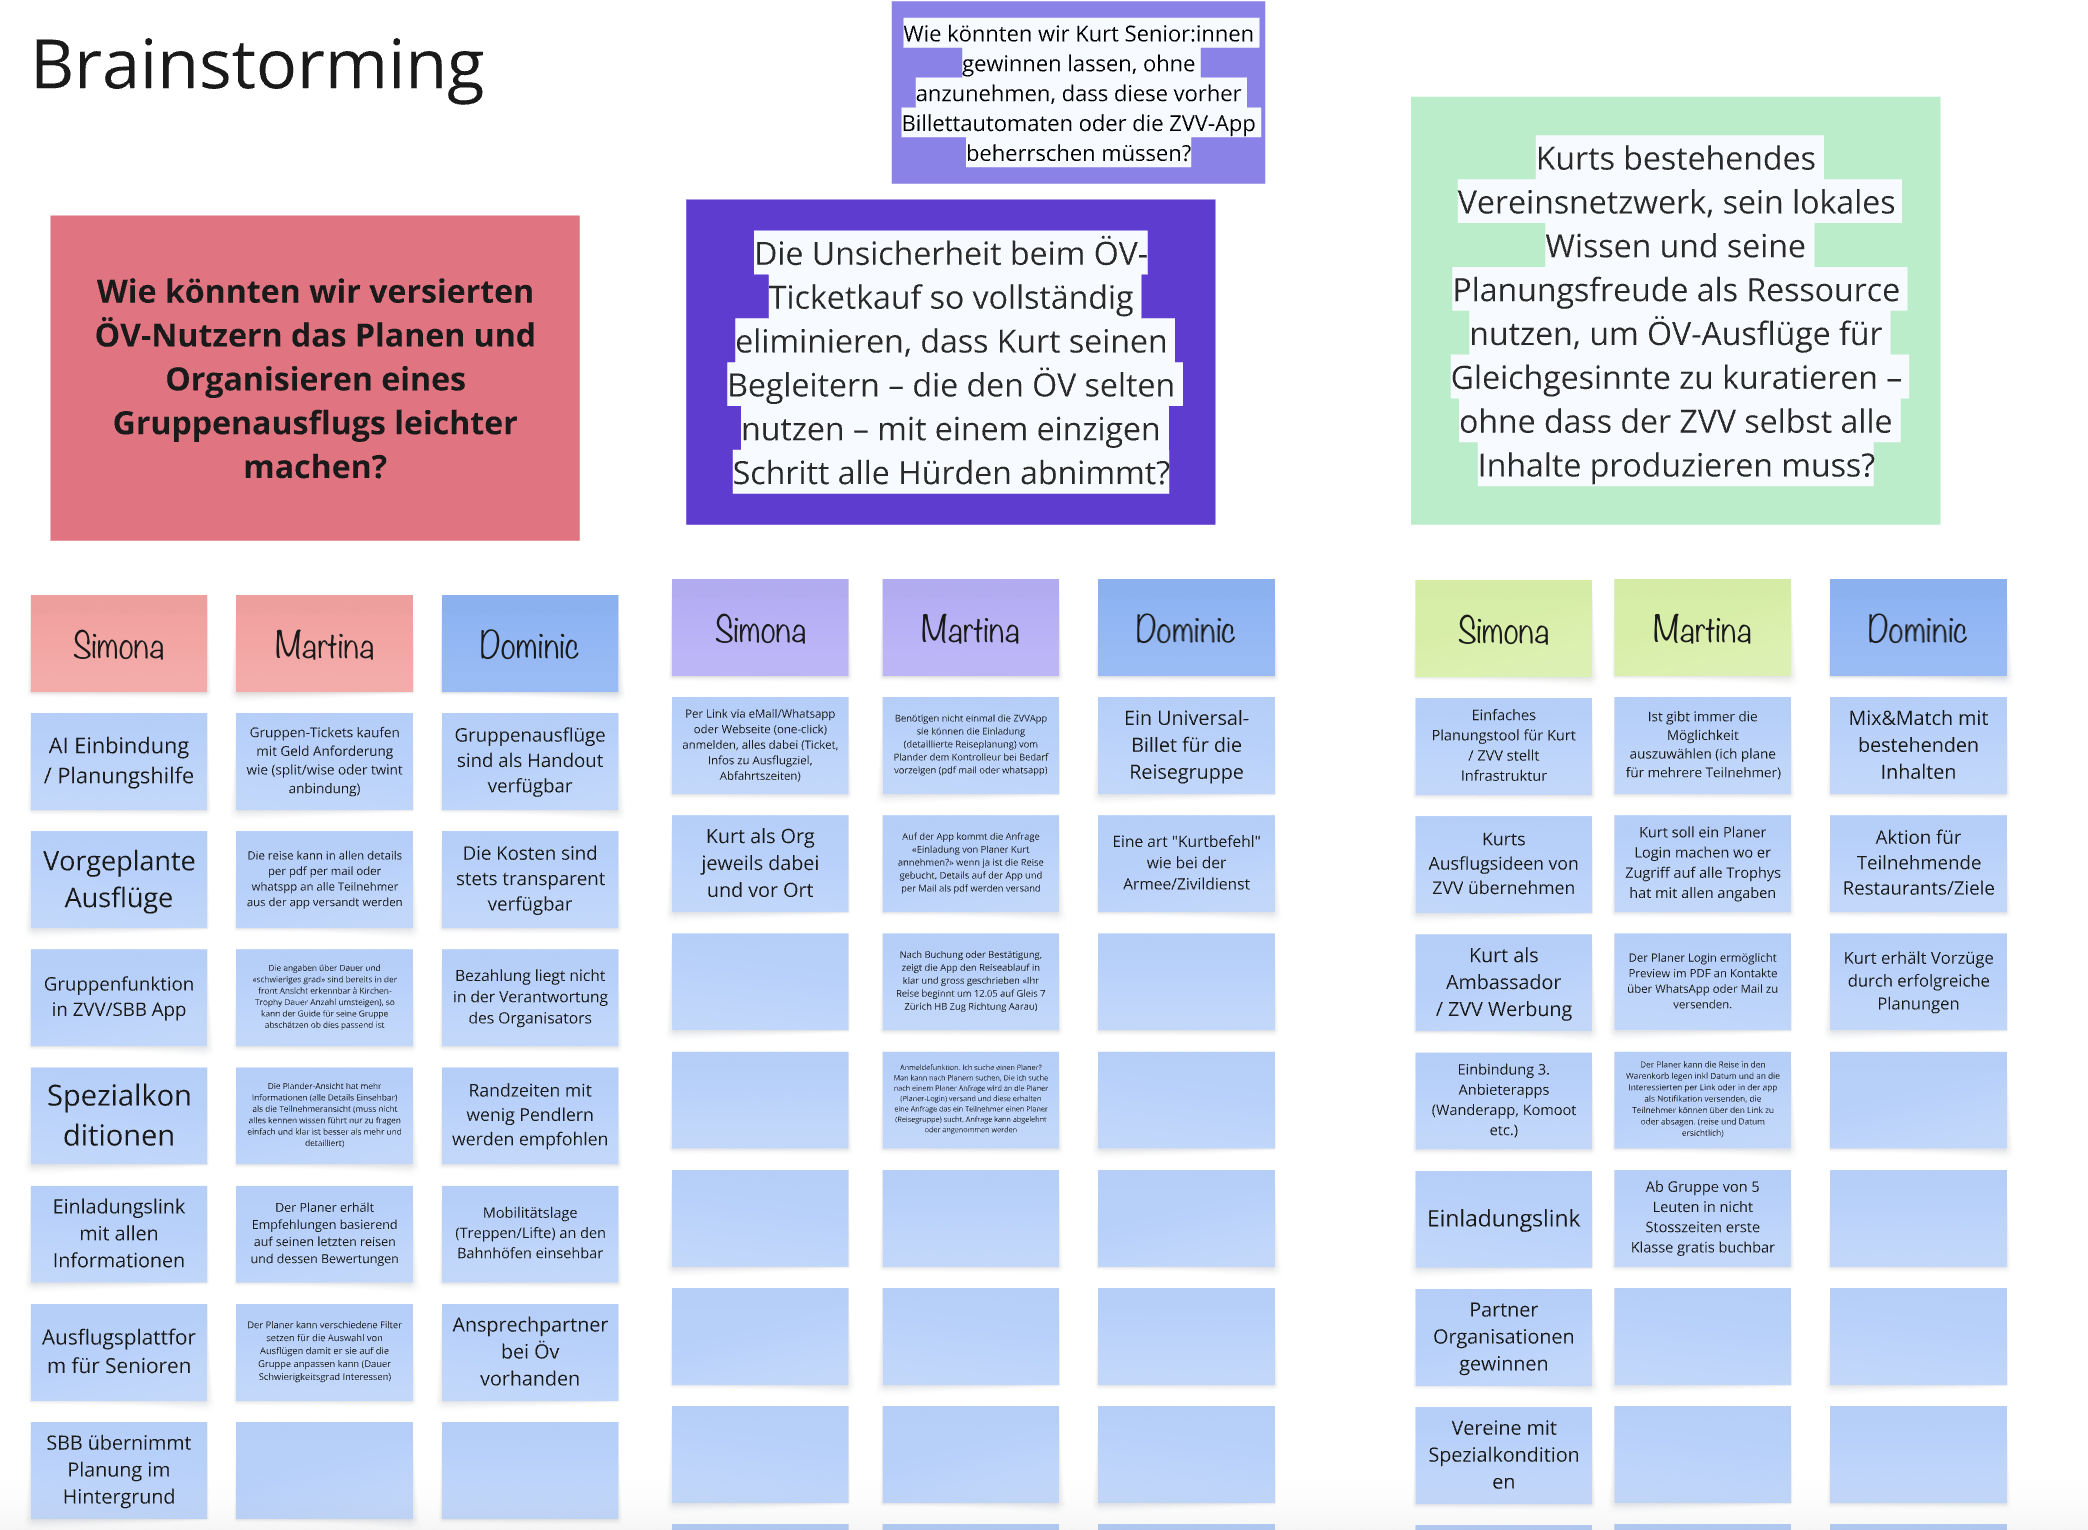
\includegraphics[width=0.72\textwidth]{ressourcen/develop/develop1.png}
\end{center}
\thispagestyle{empty}
\newpage

\printtwocolumntoc
\newpage

\pagecolor{defaultPastel}
\section{Einleitung}
\begin{multicols}{2}
\section{Einleitung}

Dieses Projekt ist als schlankes LaTeX-Grundger\"ust angelegt.

Du kannst in dieser Datei direkt Inhalte erg\"anzen oder weitere Dateien im Ordner
\texttt{sections/} anlegen und in \texttt{main.tex} einbinden.
\end{multicols}
\newpage

\pagecolor{identifyPastel}
\section{Identify Phase}
\begin{multicols}{2}
\subsection{Zweck der Identify-Phase}

Gemäss Handout ist die Identify-Phase die Orientierungsphase vor Discover.
Ziel ist es, die Ausgangslage mit dem \gls{zvv} gemeinsam zu klären, das Problemfeld zu strukturieren und ein gemeinsames Verständnis über Auftrag, Grenzen und Erkenntnisbedarf aufzubauen.

Die Phase dient damit als methodische Grundlage für den Einstieg in den ersten Diamanten (Discover/Define).
Nicht Lösungen entwickeln, sondern die Challenge präzisieren und die relevanten offenen Fragen für die Feldforschung ableiten.

\subsection{Eingesetzte Methoden und Vorgehen}

In der Identify-Phase werden vier aufeinander aufbauende Methoden eingesetzt.

\subsubsection{Challenge Deconstruction}
Die Design Challenge wird in ihre Kernbegriffe zerlegt (``Massnahmen'', ``vital'', ``autoabhängig'', ``Senior:innen'', ``Freizeitmobilität'').
Für jeden Begriff werden Assoziationen, implizite Annahmen und Spannungsfelder gesammelt und im Team verdichtet.

\subsubsection{Stakeholder Map}
Alle relevanten Akteur:innen werden in konzentrischen Kreisen erfasst: primäre Nutzende im Zentrum, danach Schlüssel-Partner und erweitertes Umfeld.
Die Methode wird genutzt, um Einflüsse auf Mobilitätsentscheidungen sichtbar zu machen und potenzielle Partner für spätere Interventionen zu identifizieren.

\subsubsection{Desk Research}
Als inhaltliche Basis werden bestehende Quellen zu Demografie, Mobilitätsverhalten, digitaler Nutzung und \gls{zvv}-Ausgangslage ausgewertet.
Verwendet werden insbesondere Bevölkerungsstatistik Kanton Zürich, Mikrozensus Mobilität und Verkehr, Mobilitätsdaten des Kantons Zürich, die Studie ``Digital Seniors'' sowie Unterlagen des \gls{zvv}.

\subsubsection{Design Space Map}
Die Ergebnisse werden abschliessend in einer Design Space Map synthetisiert.
Alle Erkenntnisse werden in drei Kategorien geordnet: ``Wir wissen'', ``Wir nehmen an'' und ``Wir wissen nicht''.
Diese Struktur dient als Brücke zur Discover-Phase und zur Schärfung des Interviewleitfadens.

\newpage
\subsection{Zentrale inhaltliche Ergebnisse}

\subsubsection{Auftrag, Zielgruppe und Rahmenbedingungen}
Der \gls{zvv} ist der grösste Verkehrsverbund der Schweiz und verfolgt drei strategische Ziele: höhere Auslastung in der \gls{nvz}, Verschiebung des Modalsplits zugunsten des \gls{oev} und nachhaltige Einstellungs- bzw. Verhaltensänderung.

Die bearbeitete Design Challenge lautet:

\begin{quote}
\textit{``Mit welchen Massnahmen können wir vitale und bislang überwiegend autoabhängige Senior:innen im Kanton Zürich zur verstärkten Nutzung des öffentlichen Verkehrs für Freizeitmobilität motivieren?''}
\end{quote}

Der Lösungsraum ist klar begrenzt.
Keine Eingriffe in Pricing, neue Tickets/Abos, Fahrplan oder Verkaufsstellen.
Im Fokus stehen Kommunikation, Services, Erlebnisse und persönliche Begleitung.

\subsubsection{Ergebnisse der Challenge Deconstruction}
Die Begriffsanalyse zeigt fünf zentrale Punkte:

\textbf{Massnahmen:} Erwartet werden keine tariflichen oder infrastrukturellen Eingriffe, sondern gestaltungsnahe Hebel im Service- und Kommunikationsraum.

\textbf{Vital:} Die Zielgruppe ist mehrheitlich selbständig, aktiv und konsumfreudig.
Gleichzeitig sehen sich viele nicht als ``Senior:innen'', was hohe Anforderungen an Sprache und Tonalität stellt.

\textbf{Autoabhängig:} Das Auto wird nicht nur als Transportmittel, sondern als Symbol für Kontrolle, Freiheit und Spontaneität verstanden.

\textbf{Senior:innen:} Keine homogene Gruppe.
Unterschiede zwischen aktiv/betagt sowie urban/ländlich und digitalaffin/offline sind für die Gestaltung zentral.

\textbf{Freizeitmobilität:} Der Nutzungskontext ist emotional und selbstgewählt.
Relevante Anlässe sind Ausflüge, Kultur, Sport, Kulinarik und Besuche.

\subsubsection{Zentrale Annahmen über die Zielgruppe}

Aus der Deconstruction verdichten sich vier Kernannahmen, die für die Gestaltung aller späteren Massnahmen zentral sind:

\textbf{Identität statt Alter:} Vitale Senior:innen sehen sich selbst oft nicht als Senioren.
Sie fühlen sich fit, aktiv und selbständig.
Diese psychologische Selbstwahrnehmung steht in Spannung zu ihrer chronologischen Zuordnung.
Folge: Sprache und Tonalität aller Kommunikation und Services muss diese Identität respektieren.
``Senioren-Angebote'' mit paternalistischem Unterton funktionieren nicht; es braucht statt dessen eine Ansprache als selbstbestimmte, erlebnisorientierte Personen.

\textbf{Autoabhängigkeit als psychologisches Phänomen:} Das Auto ist nicht bloss ein Transportmittel, sondern ein psychologisches Symbol.
Es steht für Kontrolle über Zeit, Tempo und Ziel, für Freiheit und Autonomie, für das Festhalten an Unabhängigkeit.
Diese emotionale Bindung erklärt, warum Preis- oder Angebotargumente oft nicht greifen.
Es braucht statt dessen Angebote, die das gleiche psychologische Bedürfnis (Kontrolle, Freiheit, Selbständigkeit) mit anderen Mitteln erfüllen.

\textbf{Drei unterschiedliche Segmente:} Die Zielgruppe ist heterogen nach drei Dimensionen: Lebensstil (aktiv vs. betagte), Geografie (urban vs. ländlich) und Digitalität (online vs. offline).
Diese drei Segmente haben unterschiedliche Lebenswelten, unterschiedliche Vertrauenspersonen, unterschiedliche Informationskanäle und unterschiedliche Barrieren.
Damit ist klar, dass ein ``One-Size-Fits-All''-Ansatz nicht funktioniert.

\textbf{Freizeitfahrten als Genuss und Erlebnis:} Anders als Alltagsfahrten (zur Arbeit, zum Einkaufen) sind Freizeitfahrten selbstgewählt und emotional besetzt.
Im Vordergrund stehen Genuss, Erlebnis und soziale Begegnung, nicht Effizienz oder Preis.
Das bedeutet: Ein gutes Freizeitangebot muss nicht bloss mobil versorgen, sondern eine sinnliche und soziale Erfahrung bieten.
Der Weg ist Teil des Erlebnisses, nicht bloss Mittel zum Zweck.

\subsubsection{Visualisierung der Challenge Deconstruction}
Die Mindmap basiert auf der von der Arbeitsgruppe erstellten Deconstruction-Mindmap und wird als skalierbare Vektorgrafik in LaTeX nachgebaut.
Sie verdichtet die zentralen Begriffe der Design Challenge und macht Zusammenhänge, Annahmen und Spannungsfelder auf einen Blick sichtbar.
\newpage

\FullWidthFigure[\textwidth]{sections/figures/identify_deconstruction_mindmap}{Challenge Deconstruction im \gls{zvv}-Praxis-Case (eigene Darstellung auf Basis der Gruppen-Mindmap)}

\subsubsection{Ergebnisse der Stakeholder Map}

Die Stakeholder Map erfasst alle relevanten Akteur:innen in konzentrischen Kreisen - vom Zentrum mit der Zielgruppe bis zum gesellschaftlichen Umfeld.

\textbf{Primäre Nutzende (Zentrum):}
Im innersten Kreis stehen zwei zentrale Gruppen:
Vitale, autoabhängige Senior:innen (65--79 Jahre) als Hauptzielgruppe: mobil, kaufkräftig, gewohnheitsgeprägt.
Bereits öV-fahrende Senior:innen als Referenzgruppe: wertvoll für Erfahrungsaustausch und Peer-Motivation.
Zusätzlich erfasst die Map das soziale Umfeld (Partner:in, Familie, Freunde, Kinder) als entscheidende Einflussgrösse.
Ein erstes Kernergebnis deutet sich ab: Der Mobilitätsentscheid ist oft nicht individuell - das Umfeld beeinflusst die Wahl stark.

\textbf{Schlüssel-Partner (mittlerer Kreis):}
Die Stakeholder Map identifiziert diverse Partnerorganisationen:
\gls{zvv} (Auftraggeber): Koordination, Kommunikation, Marke - aber kein direktes Fahrerlebnis.
Verkehrsunternehmen (\gls{sbb}, \gls{zsg}, weitere Verbunde): Das Fahrerlebnis entsteht hier, nicht beim \gls{zvv}.
Pro Senectute und Verein Zürcher Seniorinnen und Senioren: grösste Seniorenorganisationen mit existierendem Vertrauen und direktem Zugang.
Gemeinden und Quartierzentren: niederschwelliger physischer Zugang, besonders für Offline-Senior:innen.
Alltagsnahe Kontaktpunkte (Apotheken, Bibliotheken, Hausärzt:innen): Vertrauenspersonen im Alltag, geeignet für analoge Infovermittlung.
Freizeitanbieter: Kultur, Sport, Kulinarik, Ausflugsziele als potenzielle Kooperationspartner.
``Invisible Influencers'' (Ärzt:innen, Gemeinden, Versicherungen, Medien): prägen das gesellschaftliche Bild von Senior:innen und Mobilität, ohne selbst Angebote zu schaffen.

\textbf{Weiteres Umfeld (äusserer Kreis):}
Bund und Kantone (Regulierung, Förderung, Mobilitätspolitik).
Tourismusorganisationen (Freizeitziele und Ausflugspakete als Motivationsanker).
Autolobby (Gegenspieler im Narrativ).
Gesellschaft Schweiz (Normen rund um Mobilität, Selbständigkeit und Alter).

\textbf{Zentrale Erkenntnisse:}
Kernergebnis: Der \gls{zvv} erreicht diese Zielgruppe vermutlich nicht allein.
Partnerorganisationen mit bestehendem Vertrauen spielen eine entscheidende Rolle.
Das soziale Umfeld - Partner:in, Familie, Freunde - hat einen grösseren Einfluss auf den Mobilitätsentscheid, als die Fragestellung zunächst vermuten liess.

\FullWidthFigure[\textwidth]{sections/figures/stakeholder_map}{Stakeholder Map des \gls{zvv}-Praxis-Case (eigene Darstellung)}

\subsubsection{Ergebnisse der Desk Research}

\textbf{Methodisches Vorgehen:}
Wir sichteten die wichtigsten Schweizer Quellen zur Zielgruppe mit dem Ziel eines datengestützten Bildes: Mobilitätsverhalten, demografische Ausgangslage und digitale Nutzung - differenziert nach Segmenten, wo Daten verfügbar waren.

\textbf{Demografische Ausgangslage:}
Im Kanton Zürich leben rund 327'000 Personen über 65 Jahre (21\% der Gesamtbevölkerung), mit erwarteter Zunahme auf ca. 420'000 bis 2040 (+28\%).
Das grösste Hebelsegment sind aktive Senior:innen (65--79 Jahre): ca. 190'000 Personen, kaufkräftig mit mittlerem Nettovermögen von CHF 420'000.
Betagte Senior:innen (75--85 Jahre): ca. 107'000 Personen in Mobilitätsübergangsphase.
Offline-Senior:innen (kein Internet/Smartphone): ca. 30'000 Personen, ausschliesslich auf analoge Kanäle angewiesen.

\textbf{Mobilitätsverhalten nach Segment:}
Aktive Senior:innen (65--75 Jahre): durchschnittlich 27,4 km pro Tag - 57\% mit Auto, nur 18\% öV (CH-Ø: 23\%, Kanton Zürich ca. 22\%).
Über 60\% der Freizeitfahrten mit Auto, auch im städtischen Raum.
78\% aller Ü65 sind in der Nebenverkehrszeit unterwegs (ideal für \gls{zvv}).
Hauptmotive für Autonutzung: Flexibilität (38\%), Bequemlichkeit (27\%), kein Gepäckproblem (21\%), Sicherheitsgefühl (14\%).

Betagte Senior:innen (75--85 Jahre): durchschnittlich nur noch 11 km pro Tag - Mobilitätsradius schrumpft.
MIV-Anteil ca. 55\%, öV-Anteil steigt auf ca. 22\%.
Sicherheitsbedenken im öV: Orientierungslosigkeit, Umstiegsunsicherheit, fehlende Assistenz.

Stadt-Land-Gefälle: Stadt Zürich öV-Anteil Ü65 ca. 28\%, ländliche Gemeinden nur ca. 11\%.
Im ländlichen Raum oft stündlicher Takt und fehlende Direktverbindungen zu Freizielzielen.

\textbf{Digitale Nutzung nach Segment:}
Aktive 65--74 Jahre: 84\% Internetnutzung, 74\% Smartphone - digitale Kanäle (App, Online-Ticket) gut erreichbar.
Betagte 75--84 Jahre: 62\% Internet, 49\% Smartphone - Gap wächst, analoge Ergänzung nötig.
Offline-Senior:innen (Ø 78 J.): unter 25\% - ausschliesslich analoge Zugänge.
Hauptgründe für Nicht-Nutzung: ``zu kompliziert'' (41\%), Sicherheitsbedenken (29\%), hoher Lernaufwand (22\%).

\textbf{Der kritische Moment: Führerscheinabgabe:}
Ca. 190'000 Personen Ü65 im Kanton Zürich besitzen einen Führerausweis (ca. 80\% der Zielgruppe).
Ca. 8'000--10'000 Personen geben den Führerausweis pro Jahr ab - ein starkes Aktivierungsfenster für den öV.
Nur 34\% bereiten sich im Vorfeld mit öV-Alternativen vor.
Hauptbarrieren nach Abgabe: Orientierungslosigkeit (43\%), Sicherheitsbedenken (28\%), fehlende Information (19\%).
Bei früher Vorbereitung (mindestens 1 Jahr vorher) ist die spätere öV-Nutzungsrate signifikant höher.

\textbf{Nutzungsbarrieren für den öV:}
Psychologisch: Auto = Freiheit, Kontrolle, Spontanität; öV = Abhängigkeit. Gewohnheit über Jahrzehnte. Erste negative Erfahrung wirkt dauerhaft abschreckend. Soziale Norm: Auto dominiert im Umfeld.

Praktisch: Gepäck und Einkäufe im Auto bequemer. Wege zur Haltestelle bei Regen/Kälte als Hürde. ``Letzter Kilometer'': Freizeitziele oft nicht direkt erreichbar. öV erfordert Planung, Auto ist spontan verfügbar.

Systemisch: Tarifkomplexität, digitaler Ausschluss (Apps/Online-Tickets), abbauende physische Schalter, Stadt-Land-Gefälle bei Direktverbindungen, wenig sichtbare \gls{zvv}-Kommunikation für diese Zielgruppe.

\subsubsection{Ergebnisse der Design Space Map}

Abschliessend verdichteten wir alle Erkenntnisse in einer Design Space Map - ein dreigeteiltes Raster, das den Wissensstand systematisch offenlegt.

\textbf{Was wir wissen (Rechte Spalte):}
Züge sind nicht ausgelastet zwischen Pendlerverkehr und Nebenverkehrszeit - \gls{nvz}-Potenzial vorhanden.
Das Auto ist das Hauptfortbewegungsmittel der Zielgruppe.
\gls{zvv} hat bereits Angebote, erreicht die Zielgruppe damit aber nicht.
Die Zielgruppe ist kaufkräftig mit hohem Nettovermögen.
Die Kosten des Autos werden von der Zielgruppe oft nicht vollständig wahrgenommen.
\gls{zvv} kennt seine Kund:innen in dieser Altersgruppe kaum im Detail.
Urban gibt es guten öV-Zugang, ländlich ist der öV-Zugang deutlich schlechter.
Die Zielgruppe ist digitalaffin bei 65--74 Jahren, die Affinität nimmt ab 75 ab.

\textbf{Was wir annehmen (Mittlere Spalte):}
Das Auto steht für Freiheit, Spontanität und Selbständigkeit - nicht bloss als Transportmittel.
Physische Barrieren hemmen die öV-Nutzung: Gepäck, Wetter, schwer erreichbare Ziele (ländlich vs. Stadt).
Freizeitfahrten sind emotional besetzt und selbstgewählt, nicht zweckorientiert.
Gewohnheit schlägt rationale Entscheidung - das Auto ist die Standardwahl.
Die erste negative öV-Erfahrung (Ticket, Umstieg, Verspätung) wirkt dauerhaft abschreckend.
Social Influence ist stark: Partner:in, Freunde und Familie beeinflussen den Mobilitätsentscheid erheblich.
Die Zielgruppe sieht sich nicht als ``Senioren'' - sie fühlt sich fit und selbständig.
Beim öV entsteht Unsicherheit bei Ticket, Umstieg und Abhängigkeit vom System.

\textbf{Was wir nicht wissen (Linke Spalte):}
Gute und schlechte öV-Erfahrungen der Zielgruppe im Detail.
Konkrete Verhaltensgründe, weshalb Auto dem öV vorgezogen wird.
Typischer Tagesablauf und Freizeitprioritäten.
Informationsquellen der Zielgruppe.
Wo sie ihre Schwerpunkte setzen - die Highlight-Momente des Tages.
Wann wird überhaupt über Verkehrsmittelwahl entschieden?
Was hält sie konkret vom öV ab - was könnte sie motivieren?
Freizeitverhalten und digitale Affinität im Detail.

Mit diesem Wissensstand starteten wir die Discover-Phase.
Die offenen Fragen und Annahmen bildeten die Grundlage für den Interviewleitfaden.

\subsubsection{Visualisierung der Design Space Map}
Die Design Space Map ordnet den gesamten Wissensstand in einem dreigeteilten Raster:

\textbf{Linke Spalte -- Was wir nicht wissen:} Hier sind alle Fragen gebündelt, die für eine Aktivierungsstrategie zentral sind, aber noch offene Forschungsfragen darstellen.
Dazu gehören konkrete Gründe für die Autoabhängigkeit, Informationsquellen der Zielgruppe, situative Entscheidungslogiken, digitale Affinität und die alltägliche Routinegestaltung.

\textbf{Mittlere Spalte -- Was wir annehmen:} Basierend auf Desk Research und Teamdiskurs werden hier hypothetische Erklärungen festgehalten.
Sie beziehen sich auf psychologische Faktoren (Kontrollgefühl, Sicherheit), systemische Barriereeffekte (Erreichbarkeit, Infrastruktur) sowie soziale Einflussfaktoren.
Diese Annahmen sind bewusst gekennzeichnet und werden in der Discover-Phase empirisch überprüft.

\textbf{Rechte Spalte -- Was wir wissen:} Hier sind die gesicherten Erkenntnisse aus Sekundärdaten und Behördenkommunikation aufgeführt: die Zielgruppendemografia, die Verkehrsmittelpräferenzen, das Potenzial in der \gls{nvz} sowie die bestehende Angebotspalette des \gls{zvv}.

Die Map dient als Kompass für die kommende Feldforschung.
Sie zeigt, welche Fragen mit Interview und Beobachtung geklärt werden müssen, um von Annahmen zu verifizierten Insights zu gelangen.

\FullWidthFigure[\textwidth]{sections/figures/design_space_map}{Design Space Map des \gls{zvv}-Praxis-Case (eigene Darstellung)}

\subsection{Reflexion der Methode}

Die Kombination aus Challenge Deconstruction, Stakeholder Map, Desk Research und Design Space Map erweist sich als sinnvoll, um vom breiten Problemraum zu einem klar strukturierten Forschungsauftrag zu gelangen.
Insbesondere die Trennung in ``wissen/nehmen an/wissen nicht'' hilft, Annahmen sichtbar zu machen und nicht vorschnell als Fakten zu behandeln.

Theoretisch lässt sich dieses Vorgehen im Kontext des ``Fuzzy Front End'' verorten, das \textcite{lewrick2018} als entscheidende Weichenstellung im Design-Thinking-Prozess beschreiben.
Bevor divergent geforscht wird, muss der Problemraum eingegrenzt und das Team auf ein gemeinsames Verständnis ausgerichtet werden.
Die Design Space Map erfüllt genau diese Funktion, indem sie den Übergang vom impliziten Teamwissen zu einer expliziten, teilbaren Wissensstruktur formalisiert.

Gleichzeitig zeigt sich eine methodische Grenze der Identify-Phase.
Sie schafft Orientierung, liefert aber keine belastbare Evidenz zu Motiven und situativen Entscheidungen aus erster Hand.
Genau daraus ergibt sich der nächste Schritt im Prozess: qualitative Interviews in der Discover-Phase, um die offenen Fragen empirisch zu klären.

Rückblickend passen wir zwei Aspekte an.
Erstens versehen wir die Stakeholder Map stärker mit Hypothesen über Einflussrichtungen (z.\,B. ``Partner:in beeinflusst Verkehrsmittelwahl positiv/negativ''), um in den Interviews gezielter nachfragen zu können.
Zweitens ist der Desk Research zeitlich knapp bemessen.
Eine systematischere Literaturrecherche zu Verhaltensänderungsmodellen (etwa Transtheoretisches Modell oder Theory of Planned Behaviour) schärft die Annahmen in der Design Space Map bereits früher theoretisch.

\end{multicols}
\newpage

\pagecolor{discoverPastel}
\section{Discover Phase}
\begin{multicols}{2}
\subsection{Zweck der Discover-Phase}

Während die Identify-Phase den Problemraum aus der Vogelperspektive vermisst (\gls{deskresearch}, \gls{stakeholdermap}, \gls{designspace}), öffnet die Discover-Phase die erste Raute des \gls{doublediam} hin zur Zielgruppe selbst. Ziel ist es, die offen gebliebenen Annahmen und Wissenslücken empirisch zu prüfen und die Lebenswelt pensionierter Menschen aus erster Hand zu verstehen, also \emph{mit} der Zielgruppe zu sprechen statt \emph{über} sie.

Konkret verfolgen wir drei Erkenntnisziele: das Mobilitätsverhalten und die Entscheidungslogik zwischen \gls{miv} und \gls{oev} nachzuvollziehen, die emotionalen wie praktischen Barrieren und Motivatoren der \gls{oev}-Nutzung freizulegen sowie unsere Identify-Hypothesen zu prüfen. Die Phase ist bewusst divergent angelegt: Wir sammeln breit und unvoreingenommen, bevor in der Define-Phase verdichtet wird.

\subsection{Eingesetzte Methoden und Vorgehen}

Im Zentrum steht die qualitative Primärforschung: Wir kombinieren \gls{leitfadeninterview}s mit einem ergänzenden standardisierten Fragebogen sowie KI-generierten \emph{Synthetic Users} und werten das Material mit \gls{empathymap} und \gls{paingain} aus. Dem Profil des CAS entsprechend setzen wir gezielt KI-Werkzeuge unterstützend ein.

\subsubsection{Qualitative Leitfadeninterviews}

Als Leitmethode wählen wir das halbstandardisierte \gls{leitfadeninterview} \parencite{blume2025}, das die Innensicht der Befragten zugänglich macht. Grundregeln sind: keine Suggestiv- oder reinen Ja/Nein-Fragen, ein sparsames ``Warum?'' und stets nur eine Frage auf einmal. Die halbstandardisierte Form hält die Perspektiven vergleichbar, lässt aber Raum, unerwarteten Spuren zu folgen.

\subsubsection{Ergänzende Quellen und KI-Einsatz}

Um die qualitative Basis zu verbreitern, überführen wir den Leitfaden zusätzlich in einen standardisierten Fragebogen und verschicken ihn per E-Mail an weitere Personen der Zielgruppe. Passend zum Fokus des CAS auf \gls{designthinking} mit künstlicher Intelligenz nutzen wir generative Werkzeuge an mehreren Stellen: Claude AI als Sparringpartner beim Leitfaden, einen KI-basierten \emph{Virtual Trainer} zum Üben der Gesprächsführung sowie \emph{Synthetic Users} als KI-generierte Persona-Stellvertreter. Diese Hinweise verstehen wir bewusst als Ergänzung und nicht als Ersatz der echten Stimmen.

\subsubsection{Stichprobe, Durchführung und Synthese}

Den qualitativen Kern bilden zwei selbst geführte 30-minütige Tiefeninterviews im Rahmen der \emph{Testing Time} mit \textbf{Margrit} und \textbf{Hans Jörg}, beide pensioniert. Ergänzt um die Videointerviews der übrigen Projektteams liegen insgesamt acht Gespräche mit den beiden vor, dazu die Rückläufe aus Fragebogen und Synthetic Users. Zur Verdichtung der Rohdaten nutzen wir zwei Synthese-Werkzeuge: Die \gls{empathymap} ordnet die Aussagen in Quadranten und macht das Spannungsfeld zwischen Aussage und Verhalten sichtbar, die \gls{paingain} stellt Schmerzpunkte und Motivatoren gegenüber und bereitet die Priorisierung von Hebeln für die Develop-Phase vor.

\columnbreak
\subsection{Zentrale inhaltliche Ergebnisse}

\subsubsection{Mobilität ist Identität, nicht nur Fortbewegung}

\textbf{Das Auto steht für Freiheit und Autonomie.} Quer durch die Interviews zieht sich ein Grundmuster: ``Das Auto ist Freiheit, jederzeit einsteigen, wegfahren, ohne Fahrplan'' (Christian, Christof, Edna). Mobilität ist für die Befragten weniger eine Frage der reinen Fortbewegung als Ausdruck von Autonomie und Identität. Der \gls{oev} konkurriert damit nicht nur funktional, sondern symbolisch: Er muss aktiv ``gegen das Gewohnte'' gewählt werden, während das Auto die selbstverständliche Standardoption (``default'') bleibt. Gleichzeitig zeigt sich nach der Pensionierung eine bemerkenswerte Offenheit, ``Was kommt jetzt?'' (Peter, Christof, Hans Jörg) markiert einen biografischen Umbruch, der Raum für neue Gewohnheiten schafft.

\subsubsection{Das soziale Umfeld prägt das Verkehrsverhalten}

\textbf{Mobilität ist eine soziale Praxis.} Das unmittelbare Umfeld der Befragten ist fast ausschliesslich auto-orientiert: ``Ich kenne niemanden im Freundeskreis, der \gls{oev} fährt'' (Christian). Das erzeugt soziale Reibung und erschwert die Koordination von Ausflügen. Als Gegenkraft wirken jüngere Familienmitglieder (``Fahre doch mal mit dem Zug'') sowie Vereinskollegen, Pro Senectute und Veranstaltungskalender, die das Freizeitverhalten prägen (B.~Siegenthaler, Hans Jörg). Besonders stark ist der Wunsch nach gemeinsamem Erleben: Ausflüge mit Freundin, Gruppe oder Familie werden als sozialer Wert an sich beschrieben (Margrit, Peter).

\subsubsection{Barrieren: Wo der \gls{oev} im Alltag scheitert}

\textbf{Ticketkauf-Unsicherheit} ist die meistgenannte Hürde: ``Was, wenn ich das falsche Ticket löse?'' (P.~Büki, Margrit). Zonenfehler, eine als zu komplex empfundene App und die undurchsichtige Anschlussbillett-Logik führen bis zur Angst, ``fast als Schwarzfahrer'' dazustehen. \textbf{Das Sicherheitsgefühl} sinkt nach Einbruch der Dunkelheit, schlecht beleuchtete Bahnhöfe und ``komische Gestalten'' führen dazu, dass der \gls{oev} abends gemieden wird. \textbf{Gepäck und Transport} machen das Auto bei schweren Einkäufen, Garten- oder Werkzeugtransporten praktisch unverzichtbar. Hinzu kommen \textbf{Mitmenschen im \gls{oev}} (Lärm, Gerüche, Gedränge, fehlende Etikette) und \textbf{App-Updates}, die gelernte Bedienwege zerstören und das Vertrauen mit jeder Änderung schwächen. Die mit Abstand stärkste Barriere bleibt jedoch die \textbf{Gewohnheit}: Im Entscheidungsmoment taucht der \gls{oev} schlicht nicht als Option auf.

\subsubsection{Motivatoren: Wann der \gls{oev} überzeugt}

\textbf{Kein Parkplatzstress} ist der rationalste Treiber, ``Wenn ich nach Zürich gehe, nehme ich die S-Bahn'' (Christian, Christof), sobald das Auto zum Problem wird. Noch stärker wirken \textbf{Erlebnisfahrten}: GoldenPass, Nostalgiezug oder Dampfbahn Furka machen die Fahrt selbst zum Highlight, ``Die Fahrt ist das Ziel'' (Margrit, Hans Jörg). Für solche Erlebnisse sind die Befragten bereit zu zahlen und sorgfältig zu planen. Dazu kommen die \textbf{soziale Dimension} des gemeinsamen Unterwegsseins, die \textbf{gewonnene Zeit im Zug} (lesen, Landschaft geniessen, ohne Zeitdruck nach der Pensionierung) sowie \textbf{Natur, Wandern und Kultur} als starke Motivatoren. Bemerkenswert ist schliesslich die vorhandene \textbf{digitale Kompetenz}: Die \gls{zvv}-App wird als ``sensationell'' beschrieben (Hans Jörg, Peter), und Ausflüge werden mit Wetter-, Wanderweg- und Webcam-Apps akribisch geplant.

\columnbreak
\subsubsection{Zwei Profile im Kontrast: Hans Jörg und Margrit}

Die beiden von uns selbst geführten Interviews verdichten das Spektrum exemplarisch. \textbf{Hans Jörg fährt \gls{oev}, weil für ihn die Gewinne überwiegen}: Er erlebt die Fahrt als Teil des Ausflugs (``Bei einer schönen Strecke ist die Fahrt das Ziel''), ist digital souverän (``Die \gls{zvv}-App ist sensationell''), hat nach der Pensionierung Zeit und Musse und ist über Verein, Natur und Kultur stark an Freizeitziele gebunden, die der \gls{oev} bequem erschliesst. Die App nimmt ihm genau jene Unsicherheit, die andere abschreckt.

\textbf{Margrit fährt eher \emph{nicht} \gls{oev}, weil bei ihr die Schmerzpunkte überwiegen}: Die Ticketkauf-Unsicherheit wirkt als emotionale Hauptbarriere (``einmal stand ich fast als Schwarzfahrerin da''), und der \gls{oev} wird für sie erst attraktiv, wenn sie nicht allein unterwegs ist (``Am schönsten ist es, gemeinsam unterwegs zu sein''). Fehlt die Begleitung, überwiegen Hemmschwelle und Sicherheitsbedenken. Der direkte Vergleich zeigt: Nicht das Angebot selbst, sondern das Verhältnis von wahrgenommenen Gains und Pains entscheidet über die Nutzung.

\subsubsection{Schlüsselerkenntnis: Erlebnis schlägt Pflicht}

\textbf{Der \gls{oev} gewinnt über das Erlebnis, nicht über die Pflicht.} Die Befragten lassen sich nicht über Argumente der Vernunft oder Nachhaltigkeit aktivieren, sondern über das Versprechen eines attraktiven Freizeiterlebnisses. Wo das Auto an seine Grenzen stösst (Parkplatz, Stau) oder wo die Fahrt selbst zum Ziel wird, kippt die Entscheidung zugunsten des \gls{oev}. Diese Erkenntnis verschiebt den Fokus weg vom reinen Transportmittel hin zum Erlebnis-Zubringer.

Anhand der verdichteten Ergebnisse aus den Transkripten der Interviews wird mit Claude AI die Empathy Map und die Pain-/Gain-Map erstellt, die die Grundlage für die Define-Phase bilden.

\columnbreak
\subsection{Reflexion der Methode}

Die qualitativen \gls{leitfadeninterview}s erweisen sich als der richtige Hebel für diese Phase. Sie liefern reichhaltige, emotional aufgeladene Einblicke, die eine reine \gls{deskresearch} nicht erbringen könnte, und machen den Widerspruch zwischen Einstellung (``\gls{oev} ist mühsam'') und konkretem Verhalten (begeisterte Erlebnisfahrten) überhaupt erst sichtbar.

Gleichzeitig sind wir uns der typischen Verzerrungen bewusst, vor denen \textcite{blume2025} warnt. Dem \gls{confirmationbias}, also der Versuchung, vor allem Bestätigung für unsere Identify-Hypothesen zu suchen, begegnen wir mit bewusst offen und neutral formulierten Fragen. Dem \gls{haloeffekt} und einem \gls{ingroupbias} wirken wir entgegen, indem wir Protokolle anderer Teams einbeziehen und so unsere eigene Sichtweise relativieren.

Die Grenzen der Methode liegen in der Stichprobe: Sie ist klein, nicht repräsentativ und durch den E-Mail-Fragebogen tendenziell zu digital-affinen, aktiven Senioren verzerrt, betagte und offline lebende Personen sind unterrepräsentiert. Zudem zwingen uns technische Schwierigkeiten dazu, die Gespräche manuell statt systematisch transkribiert auszuwerten, was die Auswertungstiefe begrenzt. Auch die ergänzend befragten Synthetic Users ersetzen keine echten Menschen, da sie bestehende Annahmen reproduzieren und Verzerrungen verstärken können.

Im Rückblick würden wir die Interviews stärker durch teilnehmende \emph{Beobachtungen} ergänzen, etwa an Bahnhöfen und Ticketautomaten, um die berichtete Ticketkauf-Unsicherheit direkt im Kontext zu erfassen, und die Stichprobe gezielt um schwerer erreichbare Segmente erweitern. Für die nächste Phase liefern die verdichteten Ergebnisse aus Empathy Map und Pain-/Gain-Map die Grundlage, um Persona, \gls{pov} und How-Might-We-Fragen zu schärfen.

\FullWidthFigure{sections/figures/empathymap}{Empathy Map der frisch pensionierten Zielgruppe (65--70 Jahre) auf Basis der Leitfadeninterviews}

\FullWidthFigure{sections/figures/paingain}{Pain- und Gain-Map: Schmerzpunkte und Motivatoren der \gls{oev}-Nutzung}
\end{multicols}
\newpage

\pagecolor{definePastel}
\section{Define Phase}
\begin{multicols}{2}
\subsection{Konzept der Persona-Entwicklung}

Die Analyse der durchgeführten Interviews, der Fragebögern und Sekundärdaten bildete die Grundlage für die Erstellung von Personas. Personas sind detaillierte Archetypen von Zielnutzer:innen, die auf Forschung basieren. Sie helfen dem Team, die Perspektive der Zielgruppe zu verstehen und Lösungen nutzer-zentriert zu entwickeln.

Der Ablauf der Persona-Entwicklung war folgend:
Der Ablauf der Persona-Entwicklung folgte einer klaren Sequenz: Zuerst wurden die Interviews aus der Discovery-Phase ausgewertet und die Interviewpersonen entlang kontinuierlicher und diskreter Variablen gemappt. Darauf aufbauend erfolgte ein Clustering der Teilnehmenden, aus dem die Personas entwickelt wurden. Anschliessend wählten wir eine Leit-Persona für die vertiefte Analyse, erstellten für diese eine Customer Journey, verdichteten die Erkenntnisse in einem Point of View und leiteten daraus die How-might-we-Fragen ab.

\subsection{Persona: Kurt Kreuz und Quer}

Verdichtet aus Interviews: Reini (66), Hans Jörg (78), Peter (66)

\textit{``Standard bei mir ist die \gls{oev}. Zug, Tram, Bus, das macht doch einfach Sinn. Das Auto kommt zum Einsatz, wenn ich muss, schwere Einkäufe, spät in der Nacht ohne Anschluss. Ich bin in Vereinen tätig und gesellig, das geht im \gls{oev} halt auch am besten.''}

\subsubsection{Demografische Merkmale}

\end{multicols}

\begin{center}
\begin{tabular}{ll}
Alter & 65 bis 80 Jahre (frisch pensioniert) \\
Wohnort & Seegemeinde / städtische Agglo Zürich \\
Beruf (i.R.) & Technisch / handwerklich (Elektriker, Mechaniker, Ing.) \\
Mobilität & \gls{oev} (Freizeit \& Alltag) · Auto (Ausnahme) \\
\gls{oev}-Abo / Digital & Halbtax oder \gls{ga} · \gls{sbb}-App, \gls{zvv}-App, MeteoSwiss, WebCams
\end{tabular}
\end{center}

\begin{multicols}{2}

\subsubsection{Bedürfnisse \& Ziele}

\textbf{Bewegung \& Gesundheit:} Körperlich und geistig fit bleiben. Neues entdecken, Neues lernen, Gehirnjogging als bewusste Strategie gegen Stillstand.

\textbf{Nachhaltig handeln:} Umweltschutz ist wichtig. Möchte als Vorbild vorangehen und zeigen, dass man auch ohne Auto auskommen kann.

\textbf{Geselligkeit \& Sinnhaftigkeit:} Aktiv in Vereinen, gibt Wissen an Jüngere weiter. Enttäuscht über Ausschluss wegen Alter in manchen Kontexten.

\textbf{Entdecken \& Erleben:} Orte, Natur, Kultur, Menschen. Die Fahrt ist Erlebnis, nicht nur Transport. Wissen wird auf dem Weg gesammelt.

\subsubsection{Einstellungen}

\textbf{\gls{oev} als natürliches Default:} \gls{oev} ist erste Wahl für alle Wege. Auto kommt nur bei echtem Nutzen: schwere Einkäufe für den Garten, späte Nacht ohne Anschluss.

\textbf{Kritisch bei Komplexität:} Grundsätzlich \gls{oev}-affin, ärgert sich aber über komplizierte Zonensysteme und unlogische Ticketregeln.

\subsubsection{Verhalten}

\textbf{Tracking \& Dokumentieren:} Misst zurückgelegte Kilometer, Bergsteigungen, besuchte Orte. Sammeln und Messen ist Gewohnheit, motiviert und hält den Überblick.

\textbf{Recherche \& Eigeninitiative:} Bei unklaren \gls{oev}-Systemen wird selbst recherchiert; Ausflüge werden mit Höhenmetern und Webcams geplant, das macht Spass und hält geistig fit.

\textbf{Verantwortung \& Vorbild:} Bringt sich in Vereine ein, plant Aktivitäten mit, zeigt anderen wie es geht. Möchte Vorbild sein, auch beim Mobilitätsverhalten. ``Reini, machst du das?''

\subsection{Customer Journey: \gls{oev}-Ausflug mit der Gruppe}

Eine Customer Journey beschreibt den gesamten Weg, den eine Person durchläuft, wenn sie ein Produkt oder eine Dienstleistung nutzt, von dem Moment, wo die Idee entsteht, bis zur Nachbetrachtung des Erlebnisses. Der Begriff kommt aus dem Design Thinking und dem Marketing. Die Idee dahinter ist simpel: Man versetzt sich konsequent in die Perspektive des Nutzers, statt aus der Innenperspektive des Unternehmens zu denken.

Wir wählten die typische \gls{oev}-Nutzung der Persona ``Kurt'' ab: vom Gedanken eine Reise unternehmen zu wollen, bis zum Abschluss der Reise mit der Reflexion.

\subsubsection{Reise-Phasen und Touchpoints}

Die Journey beginnt mit der \textbf{Inspiration} aus Eigeninitiative, häufig ausgelöst durch Medien, Vereinskontexte oder Gespräche im Freundeskreis. In der anschliessenden \textbf{Koordination} entsteht bereits ein positiver sozialer Effekt, weil die Organisation gemeinsamer Aktivitäten als sinnstiftend erlebt wird. In der \textbf{Detailplanung} zeigt sich ein ambivalentes Bild: Digitale Recherche, Reservationen und Routenabgleich erzeugen Entdeckerfreude, gleichzeitig entstehen Friktionen bei Zusatzangeboten und der Integration von Bergbahn- oder Freizeitleistungen.

Besonders kritisch ist der Schritt des \textbf{Ticketkaufs}, da die Tariflogik für Gruppen als komplex und fehleranfällig wahrgenommen wird. Der \textbf{Weg zum Bahnhof} wird dagegen eher neutral bis positiv erlebt, weil Bewegung und der Verzicht auf Parkplatzsuche Vorteile bieten. Während der \textbf{Hinfahrt} überwiegen Landschaftserlebnis, Gespräche und Entspannung, wobei uneindeutige Umstiege punktuell Stress erzeugen können. Das eigentliche \textbf{Erlebnis am Zielort} ist emotional der stärkste Moment der Journey und bestätigt den Nutzen der gemeinsamen \gls{oev}-Reise.

Die \textbf{Rückreise} wird meist routinierter und ruhiger wahrgenommen, bleibt aber störungsanfällig bei Verspätungen und engen Anschlüssen. In der abschliessenden \textbf{Reflexion} dominiert Stolz auf die Organisation des Ausflugs, was als wichtiger Hebel für Wiederholung und soziale Weiterempfehlung verstanden werden kann.

\subsection{Point of View}

Basierend auf der Persona und der Customer Journey wird das Problemverständnis in einem Point of View verdichtet:

\begin{quote}
\textit{``Ich kenne den \gls{oev} in- und auswendig und merke, dass viele in meinem Umfeld gar nicht wissen, wie einfach das ist. Es macht mir Freude, andere mitzunehmen, die Route zu planen und Verantwortung zu übernehmen, damit sie einfach geniessen können. Ich möchte der Grund sein, warum jemand das nächste Mal selbst zum \gls{oev} greift.''}
\end{quote}

Zentrales Insight: Kurt ist nicht der Zielkunde, Kurt nutzt den \gls{oev} bereits. Kurt ist das Aktivierungspotenzial. Der wirkliche Zielkunde ist der Freund oder die Freundin, die Kurt überredet, mal einen Ausflug mit dem \gls{oev} zu machen. Dieses Segment zu aktivieren, durch Botschafter wie Kurt, könnte eine kritische Massnahme sein.

\subsection{How-might-we-Fragen (Impulsfragen)}

Aus der Analyse entstanden mehrere How-might-we-Fragen, die den Innovationsraum für Lösungsideen aufspannen:
Im Zentrum standen dabei sechs Leitfragen: Wie können versierte \gls{oev}-Nutzer Ausflüge für Gruppen einfacher planen und organisieren? Wie lassen sich Nicht-\gls{oev}-Nutzende so einbinden, dass sie ohne Planungsaufwand teilnehmen können? Wie kann der erste gemeinsame \gls{oev}-Ausflug so gestaltet werden, dass ein bleibender positiver Eindruck entsteht? Wie lassen sich erfahrene Nutzer:innen motivieren, als Botschafter:innen in ihrem Umfeld aktiv zu werden? Wie kann der Ankommensmoment ohne Parkplatzsuche als emotionales Plus sichtbar werden? Und wie vereinfachen wir Ticketing und Verbindungswahl für ganze Gruppen in einem Schritt?

Diese Fragen bilden den Ausgangspunkt für die Develop und Deliver Phase.

\subsection{Weitere Personas im Spektrum}

Neben Kurt Kreuz und Quer identifizierten wir zwei weitere zentrale Personas im Spektrum:

\subsubsection{Persona 2: Maria Mobil (65 bis 75 Jahre, ländlicher Raum)}

\textit{``Ich bin gerne unterwegs, aber mit dem Auto bin ich einfach flexibler. Der Bus kommt nur stündlich, und wenn ich irgendwo um 16 Uhr sein muss, schaffe ich es oft nicht.''}

\textbf{Charakteristiken:} Aktive, kaufkräftige Seniorin im ländlichen Raum. Das \gls{oev}-Angebot ist nicht attraktiv genug, lange Wartezeiten, keine Direktverbindungen. Hürde ist nicht psychologisch, sondern systemisch. Sie würde \gls{oev} nutzen, wenn das Angebot besser wäre.

\textbf{Implikation für Massnahmen:} Bei Maria braucht es nicht primär Bewusstseinswandel, sondern bessere Service-Angebote oder zielgerichtete Informationen über beste Verbindungen.

\subsubsection{Persona 3: Heinz Hüfthoch (78 Jahre, betagter Senior)}

\textit{``Seit ich nicht mehr Auto fahre, gehe ich weniger raus. Mit dem Bus bin ich unsicher, ich weiss nicht, wo ich umsteigen soll.''}

\textbf{Charakteristiken:} Betagter Senior, hat kürzlich Führerschein aufgegeben. Mobilitätsverlust ist emotionaler Schock. Hauptbarriere: Orientierungsunsicherheit, Angst vor Fehlern, Sicherheitsbedenken.

\textbf{Implikation für Massnahmen:} Heinz braucht intensive persönliche Begleitung, niederschwellige Unterstützung, und möglicherweise ein ``Buddy-System'' mit jemandem erfahrenerem. Der kritische Moment der Führerscheinabgabe ist für ihn besonders wichtig.

\subsection{Persona-Matrix und Priorisierung}

Die drei Personas spannen ein Spektrum auf:

\end{multicols}

\begin{center}
\begin{tabular}{l|l|l|l}
& Kurt (aktiv, urban, \gls{oev}-affin) & Maria (aktiv, ländlich, \gls{oev}-skeptisch) & Heinz (betagter, unsicher, Transition) \\
\hline
Alter & 65 bis 75 & 65 bis 75 & 75 bis 85 \\
Wohnort & urban & ländlich & urban/suburban \\
Status & \gls{oev}-Nutzer & Auto-Nutzer & Transition \\
Aktivierungshebel & Botschafter & Service/Info & Begleitung \\
\end{tabular}
\end{center}

\begin{multicols}{2}

Priorität für Massnahmen-Design:
Für das Massnahmen-Design priorisieren wir drei Hebel in abgestufter Reihenfolge: Erstens Kurt als Botschafter mit Multiplikatoreffekt, zweitens Maria mit Fokus auf Service-Optimierung und alltagsnahe Best-Practice-Informationen und drittens Heinz mit gezielter Begleitung im Übergang nach der Führerscheinabgabe.

\end{multicols}
\newpage

\pagecolor{developPastel}
\section{Develop Phase}
\begin{multicols}{2}
\subsection{Ideation und Lösungsraum}

Basierend auf den Erkenntnissen aus der Define Phase und den How-might-we-Fragen wurden Lösungsideen generiert, um die identifizierten Barrieren zu adressieren. Der Massnahmenraum konzentriert sich auf Kommunikation, Services, Erlebnisse und persönliche Begleitung --- den vom ZVV vorgegebenen Handlungsraum.

Der Innovationsprozess folgte dabei dem Principles of Design Thinking: Vielzahl von Ideen generieren, keine vorschnelle Bewertung, auf den Erkenntnissen der Forschung aufbauen, iterativ mit den Nutzer:innen testen.

\subsection{Drei Gestaltungsprinzipien}

Die Entwicklung von Massnahmen folgt drei übergeordneten Gestaltungsprinzipien:

\subsubsection{1. Narrativ-Shift: Auto vs. ÖV}

Das zentrale psychologische Problem ist nicht die Funktion des öV, sondern das Narrativ, das damit verbunden ist. Das Auto steht für Freiheit, Spontanität, Kontrolle, Unabhängigkeit. Der öV steht in der Wahrnehmung für Abhängigkeit, Fremdbestimmung, Einschränkung.

Gestaltungsprinzip: Umpositionierung des öV von ``notwendiges Verkehrsmittel'' (funktional) zu ``Möglichkeit für Erlebnis, Entspannung und Spontanität'' (emotionaler Benefit).

Konkret: Nicht ``Fahren Sie mit dem öV zur Kostenersparnis,'' sondern ``Fahren Sie mit dem öV und geniessen Sie Ihre Zeit --- lesen, entspannen, unterhalten.''

\subsubsection{2. Partnerschaftsmodell: Vertrauensaktivierung}

Die Stakeholder-Analyse zeigte: Der ZVV allein erreicht diese Zielgruppe nicht. Organisationen mit bestehendem Vertrauen (Pro Senectute, Gemeinden, Seniorenverbände, Apotheken, Hausärzte) spielen eine entscheidende Rolle.

Gestaltungsprinzip: Integration von Vertrauensorganisationen als Co-Aktivatoren. Diese Organisationen haben regelmässigen, niederschwelligen Zugang zur Zielgruppe und hohes Vertrauen. Sie können als Multiplikatoren fungieren.

\subsubsection{3. Transitions-Design: Führerscheinabgabe als Fenster}

Der kritische Moment der Führerscheinabgabe ist das stärkste bekannte Aktivierungsfenster für den öV. Bei früher Vorbereitung --- mindestens 1 Jahr vor der Abgabe --- ist die spätere öV-Nutzungsrate signifikant höher.

Gestaltungsprinzip: Spezielle Fokussierung auf den kritischen Moment als Aktivierungskanal. Massnahmen sollten optimal etwa 1 Jahr vor der möglichen Führerscheinabgabe (Fahrtauglichkeitsuntersuchung ab 70 Jahren) ansetzen.

\subsection{Prototyping und Testing}

Entwickelte Massnahmen wurden in Form von Low-Fidelity Prototypen (Skizzen, Szenarien, Rollenspiele) und wo möglich High-Fidelity Prototypen (funktionsfähige Services, Kampagnen-Mockups) konkretisiert. Diese wurden iterativ mit Vertreter:innen der Zielgruppe und der Partnerorganisationen getestet.

Testobjekte includeten:
Die Testobjekte umfassten Service-Szenarien (z.B. Ausflugplanung für Gruppen), Kommunikationsmaterialien und Kampagnenkonzepte sowie digitale und analoge Zugangskanäle. Zusätzlich wurden unterschiedliche Kooperationsmodelle mit Partnerorganisationen geprüft, um Umsetzbarkeit und Wirkung im Alltag früh abzusichern.

Das Feedback wurde kontinuierlich gesammelt und führte zu Anpassungen der Massnahmen.

\subsection{Dimensionen der Lösungsideen}

Aus der Ideation entstanden Lösungsansätze in mehreren Dimensionen:

\textbf{Kommunikation:} Neue Kommunikationsbotschaften und -kanäle, die das Erlebnis-Narrativ des öV stärken. Kanäle: analoge Sensibilisierung (Gemeinden, Apotheken), Mund-zu-Mund (Botschafter wie Kurt), niederschwellige Information.

\textbf{Services:} Neue Service-Angebote, die konkrete Hürden senken (z.B. Gruppen-Ticketing, Führerscheinabgabe-Begleitung, ÖV-Schnuppertage mit Guided Tours).

\textbf{Erlebnisse:} Gestaltete Erlebnisse, die den emotionalen Benefit des öV erlebbar machen (z.B. Themencafés in öV-Fahrzeugen, ÖV-Ausflugspakete mit Freizeitanbietern).

\textbf{Persönliche Begleitung:} Persönliche Support-Angebote für Transitionen (z.B. Buddy-Systeme, ÖV-Navigations-Support für Erstnutzende).

\subsection{Messbarer Erfolg}

Für das Prototyping wurden bereits Erfolgskriterien definiert:
Im Mittelpunkt standen die Teilnehmendenzahl und die Regelmässigkeit der öV-Nutzung, die Zufriedenheit mit den getesteten Formaten, die Conversion von Schnupper- zu Dauerangeboten sowie Weitergabeeffekte über Mund-zu-Mund-Kommunikation durch Botschafter:innen. Ergänzend wurde die Qualität der Zusammenarbeit mit Partnerorganisationen als eigener Erfolgsfaktor erfasst.

\subsection{Konkrete Lösungsbeispiele}

Aus der Ideation entstanden mehrere konkrete Lösungskonzepte, die in der Pilot-Phase getestet werden:

\subsubsection{Beispiel 1: ``ÖV-Botschafter-Programm''}

Eine strukturierte Initiative, um Personen wie Kurt zu aktivieren und auszubilden:
Das Programm beginnt mit der Rekrutierung aktiver ÖV-Nutzer:innen über bestehende Abos, Vereinsstrukturen und Befragungen. Darauf folgt ein kompaktes Training zu Mobilitätsrecht, Systemsicherheit und dem Umgang mit unsicheren Erstnutzenden. In der Aktivierungsphase laden Botschafter:innen ihr Umfeld zu begleiteten Schnupperfahrten ein und erhalten dafür passendes Material. Kleine Anreize wie Rabatte oder Community-Events unterstützen die Motivation, während regelmässige Austauschformate den Wissenstransfer und die Qualität sichern.

Ziel: Erreiche 30--50 Botschafter pro Pilotgemeinde, jede/r aktiviert durchschnittlich 3--5 neue Nutzer:innen.

\subsubsection{Beispiel 2: ``Führerscheinabgabe-Begleitung''}

Ein systematisches Programm für den kritischen Moment der Führerscheinabgabe:
Das Programm setzt früh an, indem Informationsmaterial etwa ein Jahr vor einer möglichen Führerscheinabgabe über Hausärzt:innen und Behörden verteilt wird. Kernstück ist ein Coaching mit fünf bis sechs Kontakten: einem Einstiegskurs zum Systemverständnis, mehreren begleiteten Fahrten mit schrittweiser Selbstständigkeit, einer ersten eigenständigen Fahrt und einer strukturierten Nachbesprechung. Anschliessend werden die Teilnehmenden an bestehende öV-Netzwerke, Vereine und Gruppen angebunden, damit neue Routinen sozial stabilisiert werden.

Ziel: Von den Personen, die einen Führerschein abgeben, nutzen mindestens 50\% regelmässig den öV.

\subsubsection{Beispiel 3: ``Gruppen-Ticketing und ÖV-Ausflugspakete''}

Service-Verbesserung für die häufige Use Case von Freizeitfahrten in Gruppen:
Für Gruppenreisen wurde ein Serviceansatz entwickelt, der ein einfaches App- oder Web-Ticketing mit transparenten Tarifen und automatischer Best-Deal-Logik verbindet. Ergänzend sollen Kooperationen mit Freizeitanbietern vorgepackte Ausflugspakete ermöglichen, während Gruppenrabatte den Einstieg erleichtern und den wahrgenommenen Planungsaufwand reduzieren.

Ziel: Reduktion des Planungs-Pain-Points ``Ticketing für Gruppen''.

\subsubsection{Beispiel 4: ``Analoge Schnellstart-Kits für Offline-Senior:innen''}

Für die ca. 30\% Offline-Senior:innen, die nicht digital erreichbar sind:
Für nicht-digitale Zielgruppen setzt das Schnellstart-Kit auf physische Verteilungspunkte wie Apotheken, Gemeindezentren und Arztpraxen. Inhaltlich kombiniert es eine gedruckte Einstiegshilfe zum Ticketkauf mit Netzkarte und alltagsnahen Zielbeispielen samt Fahrplänen; ergänzt wird dies durch eine Hotline und Vor-Ort-Unterstützung über Partnerorganisationen.

Ziel: Niederschwelliger Zugang für nicht-digitale Zielgruppe.

\subsection{Testing-Ansätze und Iteration}

Die vier Lösungskonzepte wurden in niedrig- und hochfidelity Prototypen getestet:

\subsubsection{Low-Fidelity Testing: Szenarien und Rollenspiele}

Mit Vertreter:innen der Personas wurden Szenarien durchgespielt:

\textit{Szenario 1: Kurt möchte einen Ausflug für Gruppe organisieren}
Ausgangslage war ein geplanter Säntis-Ausflug mit sechs Vereinskollegen. Die Kette aus Inspiration (Vereinsmail), Koordination (Telefon), Planung (interaktive Routen- und Kostenübersicht) und Ticketing zeigte klar: Der grösste Pain Point liegt in der Ticketkomplexität für Gruppen. Eine One-Click-Lösung mit automatischer Tarifoptimierung wurde in allen Durchläufen als potenzieller Game-Changer bewertet.

\textit{Szenario 2: Maria (ländlich) plant Besuch im Kunstmuseum}
Bei Maria wurde sichtbar, dass nicht primär der Wille, sondern die wahrgenommene Unsicherheit bei Taktung und Verbindungslogik hemmt. Eine visuell geführte Informationsseite mit Kartenbild, Fahrplanpfad und konkreten Optionen reduzierte die Hürde deutlich stärker als textlastige Zoneninformationen.

\textit{Szenario 3: Heinz nach Führerscheinabgabe}
Im dritten Szenario stand Heinz nach Führerscheinabgabe vor seiner ersten selbst organisierten Zugfahrt zu den Enkeln. Das Zusammenspiel aus Buddy-Begleitung, kurzem telefonischem Vorab-Support, Erinnerung vor der Fahrt und Check-in danach zeigte, dass emotionale Sicherheit mindestens so wichtig ist wie reine Sachinformation.

\subsubsection{High-Fidelity Testing: Prototypen mit Partner:innen}

Mit ausgewählten Partnerorganisationen wurden Materialien und Services getestet:
Mit ausgewählten Partnerorganisationen testeten wir ein ÖV-Botschafter-Handbuch inklusive Trainingsunterlagen, Mockups für digitales Gruppen-Ticketing, gedruckte Schnellstart-Kits für Offline-Senior:innen sowie Workshop-Formate zur Partneraktivierung. Das Feedback fiel überwiegend positiv aus und führte vor allem zu Vereinfachungen in Sprache, Prozessschritten und Übergabepunkten.

Das Feedback war durchgehend positiv, mit wichtigen Anpassungen zur kulturellen Angepasstheit und zur Vereinfachung der Prozesse.

\end{multicols}
\newpage

\pagecolor{deliverPastel}
\section{Deliver Phase}
\begin{multicols}{2}
\subsection{Zweck der Deliver-Phase}

Die Deliver-Phase bildet den zweiten Teil des zweiten Diamanten und überführt die in der Develop-Phase entwickelten Prototypen in eine validierte Stossrichtung \parencite{designcouncil2005}. Während die Develop-Phase den Lösungsraum geöffnet und das Konzept \enquote{ZVV Tageserlebnis} erfahrbar gemacht hat, beantwortet die Deliver-Phase die Frage \enquote{Trägt die Lösung wirklich?}. Im Zentrum steht damit das Testen der Annahmen, auf denen das Konzept beruht: Akzeptanz, Preisbereitschaft und digitale Hürden.

Methodisch folgt die Phase dem Grundsatz, einen Prototyp zu bauen, als hätte man recht, ihn aber zu testen, als läge man falsch \parencite{leifer2015}. Nicht die Bestätigung der eigenen Idee ist das Ziel, sondern das frühe Aufdecken von Schwachstellen, solange Anpassungen noch günstig sind. Die Prototypen aus der Develop-Phase konfrontieren wir dafür mit echten Nutzenden aus der Zielgruppe und werten sie systematisch aus \parencite{zhaw2026testing}.

\subsection{Eingesetzte Methoden und Vorgehen}

\subsubsection{Qualitativer Prototypentest}
Zur Validierung führen wir am 19.~Juni 2026 zwei qualitative Prototypentests durch. Getestet werden drei Prototypen des Gesamtkonzepts: die \textbf{Planer-App} für den Gastgeber, die \textbf{Anmelde-App} für die eingeladenen Teilnehmenden sowie die \textbf{Treffpunkt-Idee \enquote{Donnerstags mit Kurt}}. Jeder Test folgt einem strukturierten \gls{leitfadeninterview} mit einem festen Ablauf: einer Einführung ins Projekt, einem kurzen Video zur Einstimmung, anschliessend je einer kurzen Demo der beiden Apps und zuletzt der Vorstellung der Treffpunkt-Idee über Plakat und Website. Zu jedem Prototyp stellen wir dieselbe Abfolge offener Fragen: ob die Person die Lösung nutzen würde, was ihr gefällt, was nicht und welche Alternativen ihr einfallen.

\subsubsection{Auswahl der Testpersonen}
Als Testpersonen wählen wir bewusst zwei pensionierte ehemalige Lehrpersonen aus, \textbf{Lisbeth} (68) und \textbf{Enrico}, genannt Rico (71). Der Auswahl liegt die Annahme zugrunde, dass sich Lehrpersonen im Berufsleben überdurchschnittlich häufig mit der Organisation von Gruppenreisen befassen, etwa Klassenlagern, Exkursionen und Schulreisen, und daher der Gastgeber- und Planerrolle der Persona Kurt besonders nahe stehen. Zugleich decken die beiden zwei gegensätzliche Reisetypen ab: Lisbeth ist reisefreudig, ein ausgesprochener Gruppenmensch und plant gerne für ihre Familie, während Rico ein Einzelgänger ist, am liebsten allein reist und den \gls{oev} mangels Halbtax als zu teuer empfindet. So lassen sich sowohl die Sicht potenzieller Gastgeber als auch die kritische Aussenperspektive abbilden.

\subsubsection{Feedback Capture Grid}
Zur Auswertung nutzen wir je Prototyp ein \gls{feedbackgrid}. Dieses ordnet alle Rückmeldungen in vier Quadranten, \textbf{Positiv}, \textbf{Optimieren}, \textbf{Fragen} und \textbf{Ideen}, und macht die Beobachtungen so über beide Testpersonen hinweg vergleichbar \parencite{zhaw2026testing}. Aussagekräftige Originalzitate ordnen wir den jeweiligen Personen zu, um die Befunde nachvollziehbar zu belegen.

\newpage
\subsection{Zentrale inhaltliche Ergebnisse}

\subsubsection{Prototyp 1: Planer-App}
Die Planer-App stösst bei beiden Testpersonen auf sofortige Begeisterung: Den Aufbau erleben sie als klar und verständlich, die App-Idee erfassen sie schnell. Besonders treffend ist Lisbeths Vergleich, die App sei \enquote{wie ein Doodle, aber für eine Reise}, bei der die Teilnehmenden alles auf einen Blick sehen. Ausdrücklich loben beide die Erinnerungsfunktion und die Übersicht, wer sich angemeldet hat, den sichtbaren Preis als wichtiges Informationselement sowie die Wissens- und Geschichtsinhalte der Touren als erkennbaren Mehrwert (\enquote{Überall ist Wissen, das finde ich gut}, Rico). Bemerkenswert ist Ricos Einordnung der Kostenfrage: \enquote{Wenn so ein Erlebnis dahinter ist, würde ich bezahlen}, der \gls{oev}-Preis ist kein Hindernis, sofern das Erlebnis stimmt.

Im Quadranten \emph{Optimieren} zeigen sich konkrete Verbesserungswünsche: eine flexibel wählbare Startzeit (nicht jeder kann um 09:00~Uhr starten), ein flexibler Einstiegsbahnhof (nicht alle kommen aus Zürich), eine begrenzbare Teilnehmerzahl von rund 15 Personen, ein klarer Hinweis auf den Preis für Vollzahler ohne Halbtax sowie eine deutlichere Beschreibung des Ticket-Inhalts. Offen bleiben Fragen nach der Angabe von Verpflegungswünschen, nach dem Zugang ohne Smartphone und danach, ob direkt in der App gebucht oder nur geplant wird.

\subsubsection{Prototyp 2: Anmelde-App}
Die Anmelde-App aus Sicht der eingeladenen Teilnehmenden überzeugt durch ihre Übersichtlichkeit: \enquote{Sehr gut, gute Übersicht, man weiss genau, was man da macht} (Lisbeth). Lisbeth würde die App nutzen und sie als Vereinfachung des Einladens von Freunden und Familie schätzen. Auch Rico, der selbst lieber allein reist, erkennt den Wert für sein Umfeld klar an: \enquote{In meinem Umfeld würden es viele machen, das weiss ich}.

Im Zentrum der Optimierungspunkte steht der Bezahlprozess, der für beide unklar bleibt (\enquote{Wie zahle ich per Twint? Mir ist nicht klar, wie bezahlt wird}, Lisbeth), ergänzt um den erneuten Wunsch nach einer klar ausgewiesenen Halbtax-Variante und einem verständlicheren Ticket-Inhalt. Aus den offenen Fragen ragt eine besonders heraus: ob Kurt am Treffpunkt mit dem Geldeinzug beschäftigt sei, \enquote{Würde ich mir fragen, ob Kurt die erste halbe Stunde damit beschäftigt ist, Geld einzuziehen} (Lisbeth). Daraus entsteht die übereinstimmende Idee beider, die Bezahlung vollständig vorab und digital zu lösen, kein Bargeld am Treffpunkt, sowie Verpflegungswünsche bereits bei der Anmeldung zu erfassen.

\subsubsection{Prototyp 3: Treffpunkt \enquote{Donnerstags mit Kurt}}
Der wöchentliche Offline-Treffpunkt am Zürcher Hauptbahnhof ist der klare Favorit beider Testpersonen. Das Konzept verstehen beide sofort und bewerten es als gute Idee, Rico sieht ein deutliches Potenzial gerade für Pensionierte, die allein oder frisch pensioniert sind. Der niederschwellige, gesellige Charakter überzeugt, weil er Menschen ausserhalb des eigenen Umfelds zusammenbringt.

Zugleich nennen beide klare Bedingungen: Das Programm müsse vorab transparent sein (\enquote{nicht hingehen, ohne zu wissen wohin}), die Bezahlung müsse geklärt sein, damit Kurt nicht am Treffpunkt Geld einziehen muss, und statt eines QR-Scans brauche es einen einfachen Klick-Link. Damit bestätigt der dritte Prototyp die übergreifende Tendenz: Der soziale, physische Anker trägt am stärksten, sofern Information und Bezahlung im Vorfeld gelöst sind.

\subsubsection{Vier zentrale Erkenntnisse}
Über alle drei Prototypen hinweg verdichten sich die Beobachtungen zu vier Erkenntnissen:

\begin{description}
  \item[1. Vorinformation ist Pflicht.] Niemand fährt blind los. Ziel, Programm, Treffpunkt, Preis und Verpflegung müssen vorab klar kommuniziert sein.
  \item[2. Der Treffpunkt zündet am stärksten.] Das niederschwellige Donnerstags-Format spricht Pensionierte am meisten an und bringt Fremde zusammen.
  \item[3. Digital darf keine Hürde sein.] QR-Code, App und Online-Zahlung überfordern viele in der Zielgruppe. Es braucht den einfachen Link und stets auch einen analogen Weg.
  \item[4. Kurt ist der Schlüssel, entlastet ihn.] Der vertraute Gastgeber macht den Unterschied. Tickets und Bezahlung dürfen ihn aber nicht aufhalten, und seine Spesen müssen gedeckt sein.
\end{description}

\subsubsection{Mehrwert für den ZVV}
Aus den bestätigten Annahmen lässt sich der Nutzen für den \gls{zvv} klar benennen. Tagesausflüge füllen \textbf{freie Sitze in den Nebenzeiten} unter der Woche und ausserhalb des Pendelverkehrs, ohne zusätzliche Infrastruktur-Investition. Das Angebot erschliesst eine \textbf{neue Zielgruppe 65+}, die sonst selten den \gls{oev} nutzt, und bindet sie als regelmässige Kundschaft. Es stiftet zugleich einen \textbf{gesellschaftlichen Wert}, indem es gegen Vereinsamung wirkt und ältere Menschen aktiv hält, was direkt auf die Marke einzahlt. Und es hat eine \textbf{niedrige Einstiegshürde}, weil es auf dem bestehenden Netz und Tarif aufbaut und damit in rund drei Monaten pilotfähig wäre.

\subsubsection{Nächste Schritte}
Aus den Tests leiten wir einen vierstufigen Weg vom Prototyp zum Pilotbetrieb ab:

\begin{enumerate}
  \item \textbf{Pilot mit drei Touren} in einer Region mit ausgewählten Gastgebern und echtem Feedback der Zielgruppe.
  \item \textbf{Integration des \gls{oev}-Tickets}, also die saubere Anbindung des Festpreis-Pakets an Tarif und Buchung des \gls{zvv}.
  \item \textbf{Touren ausbauen} mit weiteren Themen, Bausteinen und Regionen.
  \item \textbf{Rollout im Kanton} als festes Angebot mit vielen Gastgebern und vollen Wochentagen.
\end{enumerate}

\subsection{Dokumentation der Feedback Capture Grids}
Die folgenden drei Raster dokumentieren die Rohrückmeldungen beider Testpersonen je Prototyp, geordnet nach den vier Quadranten des \gls{feedbackgrid}. Sie bilden die Grundlage der oben verdichteten Ergebnisse. Kürzel: \textbf{L}~=~Lisbeth, \textbf{R}~=~Rico, \textbf{Beide}~=~übereinstimmende Aussage.

\end{multicols}

\newpage
\begin{center}\textbf{Prototyp 1: Tagestouren-App (Planer-App mit fertig zusammengestellten Ausflügen)}\end{center}
\FeedbackGrid
{% Positiv
\begin{itemize}[nosep,leftmargin=1.3em]
  \item Sofortige Begeisterung, klare Übersicht, Idee schnell erfasst \textbf{(L\,\&\,R)}
  \item \enquote{Wie ein Doodle, aber für eine Reise}, alles auf einen Blick \textbf{(L)}
  \item Sichtbarer Preis als wichtiges Info-Element \textbf{(L)}
  \item Wissensinhalte als Mehrwert: \enquote{Überall ist Wissen} \textbf{(R)}
  \item ÖV-Preis kein Hindernis: \enquote{Mit Erlebnis dabei, würde ich bezahlen} \textbf{(R)}
\end{itemize}}
{% Optimieren
\begin{itemize}[nosep,leftmargin=1.3em]
  \item Startzeit flexibel wählbar, nicht jeder startet um 09:00 \textbf{(L)}
  \item Einstiegsbahnhof flexibel, nicht alle kommen aus Zürich \textbf{(R)}
  \item Datumsvorschläge im Doodle-Stil anbieten \textbf{(L)}
  \item Teilnehmerzahl limitierbar, max.~15 Personen \textbf{(R)}
  \item Ticket-Inhalt klarer: was ist inklusive (Essen, Eintritt)? \textbf{(R)}
\end{itemize}}
{% Fragen
\begin{itemize}[nosep,leftmargin=1.3em]
  \item Verpflegungswünsche angebbar (vegetarisch, kein Mittagessen)? \textbf{(R)}
  \item Zugang zum Ticket ohne Smartphone? \textbf{(L)}
  \item Tour passend zur Fitness der Gruppe wählen? \textbf{(R)}
  \item Direkt in der App gebucht oder nur geplant? \textbf{(L)}
\end{itemize}}
{% Ideen
\begin{itemize}[nosep,leftmargin=1.3em]
  \item Mitteilungsfeld für individuelle Wünsche bei der Anmeldung \textbf{(L)}
  \item Routen anpassbar: Einstieg ab beliebiger Haltestelle \textbf{(L)}
  \item Mehrere Abfahrtszeiten pro Tour als Optionen \textbf{(L)}
  \item Touren auch für Haustiere (Hunde), Nischenidee \textbf{(L)}
\end{itemize}}
\captionof{figure}{Feedback Capture Grid, Prototyp~1: Tagestouren-App}

\bigskip
\begin{center}\textbf{Prototyp 2: Gruppenreise-App (Teilnehmer-Ansicht und Buchungsflow)}\end{center}
\FeedbackGrid
{% Positiv
\begin{itemize}[nosep,leftmargin=1.3em]
  \item Gute Übersicht: \enquote{man weiss genau, was man da macht} \textbf{(L)}
  \item Vereinfacht das Einladen von Freunden und Familie, \enquote{würde es auf jeden Fall nutzen} \textbf{(L)}
  \item Wert fürs Umfeld anerkannt: \enquote{In meinem Umfeld würden es viele machen} \textbf{(R)}
\end{itemize}}
{% Optimieren
\begin{itemize}[nosep,leftmargin=1.3em]
  \item Bezahlprozess unklar: \enquote{Wie zahle ich per Twint?} \textbf{(L)}
  \item Ticket-Inhalt klarer kommunizieren, ein Sternchen reicht nicht \textbf{(R)}
  \item Halbtax-Variante separat ausweisen \textbf{(L)}
\end{itemize}}
{% Fragen
\begin{itemize}[nosep,leftmargin=1.3em]
  \item Ist Kurt am HB mit Geldeinzug beschäftigt? \enquote{\dots die erste halbe Stunde Geld einziehen} \textbf{(L)}
  \item Wie wird die Buchung bestätigt, Ticket per SMS oder selbst lösen? \textbf{(L)}
\end{itemize}}
{% Ideen
\begin{itemize}[nosep,leftmargin=1.3em]
  \item Verpflegungswünsche bereits bei der Anmeldung erfassen \textbf{(L)}
  \item Bezahlung komplett vorab digital, kein Bargeld am Treffpunkt \textbf{(Beide)}
  \item Maximale Gruppengrösse 12--15, danach ein zweiter Guide \textbf{(R)}
\end{itemize}}
\captionof{figure}{Feedback Capture Grid, Prototyp~2: Gruppenreise-App}

\bigskip
\begin{center}\textbf{Prototyp 3: \enquote{Donnerstags mit Kurt}, Offline-Treffpunkt Zürich HB}\end{center}
\FeedbackGrid
{% Positiv
\begin{itemize}[nosep,leftmargin=1.3em]
  \item Konzept klar verstanden, gute Idee, \enquote{gerade für aktive Rentner} \textbf{(L)}
  \item Potenzial für allein oder frisch Pensionierte: \enquote{wie Wandergruppen, einfach mit ÖV} \textbf{(R)}
  \item Offenheit für Fremde: \enquote{mitgehen, um neue Leute kennenzulernen} \textbf{(L)}
  \item HB und Kiosk als natürlicher Sammelpunkt bestätigt \textbf{(L\,\&\,R)}
  \item Rico würde selbst ein \enquote{Kurt} werden, max.~12, Reise gratis \textbf{(R)}
  \item Erwartung an Kurt: Wissen, Geschichten erzählen, Lernen ermöglichen \textbf{(L)}
\end{itemize}}
{% Optimieren
\begin{itemize}[nosep,leftmargin=1.3em]
  \item Vorabinformation zwingend, nicht \enquote{blind} auftauchen \textbf{(L)}
  \item Bezahlprozess vorab klären \textbf{(L)}
  \item QR-Code wird nicht gescannt~$\rightarrow$~einfacher Weblink/URL \textbf{(R)}
  \item Werbung gezielt platzieren: Facebook, WhatsApp, Gemeindeanlässe \textbf{(R)}
  \item Recruiting-Film auf Mundart sprechen \textbf{(R)}
  \item Video länger und erklärender gestalten \textbf{(R)}
\end{itemize}}
{% Fragen
\begin{itemize}[nosep,leftmargin=1.3em]
  \item Bezahlung am Treffpunkt: Twint, Cash oder vorab? \textbf{(L)}
  \item Wie wird man offiziell ein \enquote{Kurt}, Anmeldung, Vorbereitung? \textbf{(R)}
  \item Wie viele Donnerstags-Ziele pro Monat, wie weit voraus sichtbar? \textbf{(L)}
  \item Treffpunkt auch in anderen Städten (Luzern, Bern)? \textbf{(L)}
\end{itemize}}
{% Ideen
\begin{itemize}[nosep,leftmargin=1.3em]
  \item Online-Kalender mit allen Donnerstags-Zielen (ohne App) \textbf{(L)}
  \item Facebook und WhatsApp als Hauptkanal für 65+ \textbf{(R)}
  \item Distribution über Gemeinde-Newsletter und Rentnerveranstaltungen \textbf{(R)}
  \item Ausweitung auf Luzern, Bern, Winterthur \textbf{(L)}
\end{itemize}}
\captionof{figure}{Feedback Capture Grid, Prototyp~3: \enquote{Donnerstags mit Kurt}}

\begin{multicols}{2}

\subsection{Reflexion der Methode}

Der Prototypentest bestätigt den Wert des testorientierten Mindsets: Erst die Konfrontation mit echten Nutzenden macht sichtbar, dass nicht die Apps, sondern der physische Treffpunkt am stärksten trägt, und dass die digitale Bezahlung eine ernsthafte Hürde darstellt. Beide Befunde sind aus der reinen Konzeptarbeit nicht ableitbar und korrigieren die ursprüngliche, app-zentrierte Erwartung. Das Feedback Capture Grid erweist sich dabei als wirksames Werkzeug, um die Fülle an Rückmeldungen strukturiert und vergleichbar zu verdichten.

Kritisch einzuordnen ist die geringe Stichprobe von nur zwei qualitativen Tests, die keine repräsentativen Aussagen erlaubt und erste Tendenzen statt belastbarer Häufigkeiten liefert. Hinzu kommt, dass die Prototypen teils nur telefonisch gezeigt werden können, was die Demo einschränkt, und dass die Auswahl ehemaliger Lehrpersonen auf einer plausiblen, aber nicht validierten Annahme über deren Nähe zur Gastgeberrolle beruht. Die Tests ersetzen daher keinen Feldtest, sondern schärfen die Richtung: Die abgeleiteten nächsten Schritte überführen die offenen Punkte, allen voran die Vorab-Bezahlung und der niederschwellige Zugang, in einen echten Pilotbetrieb, in dem sie mit einer grösseren und breiteren Gruppe validiert werden.

\end{multicols}

\newpage
\pagecolor{defaultPastel}
\markboth{Glossar und Abkürzungsverzeichnis}{Glossar und Abkürzungsverzeichnis}
\section*{Glossar und Abkürzungsverzeichnis}
\addcontentsline{toc}{section}{Glossar und Abkürzungsverzeichnis}
\printglossary[title=Glossar,nonumberlist]
\printglossary[type=\acronymtype,title=Abkürzungsverzeichnis]

\newpage
\pagecolor{defaultPastel}
\markboth{Literaturverzeichnis}{Literaturverzeichnis}
\section*{Literaturverzeichnis}
\addcontentsline{toc}{section}{Literaturverzeichnis}
\nocite{*}
\printbibliography[heading=none]

\pagecolor{defaultPastel}

\end{document}